\TNchapter[The agent you benchmarked in March is not the agent you have in June. Models update. Prompts drift. The benchmark itself becomes stale. This chapter is about what changes when you move from a one-off pick to a continuous comparison: regression benchmarking, version-aware leaderboards, hand-in-glove human-in-the-loop checks, and the open secret of public leaderboards --- that they get gamed. It closes Part III with the statistical discipline that distinguishes a real regression from noise, so your team can tell, on Monday, whether last week's release actually got worse.]{Comparing agents over time}
\label{ch:30-benchmarking-12-comparing}

\begin{figure*}[tb]
\centering
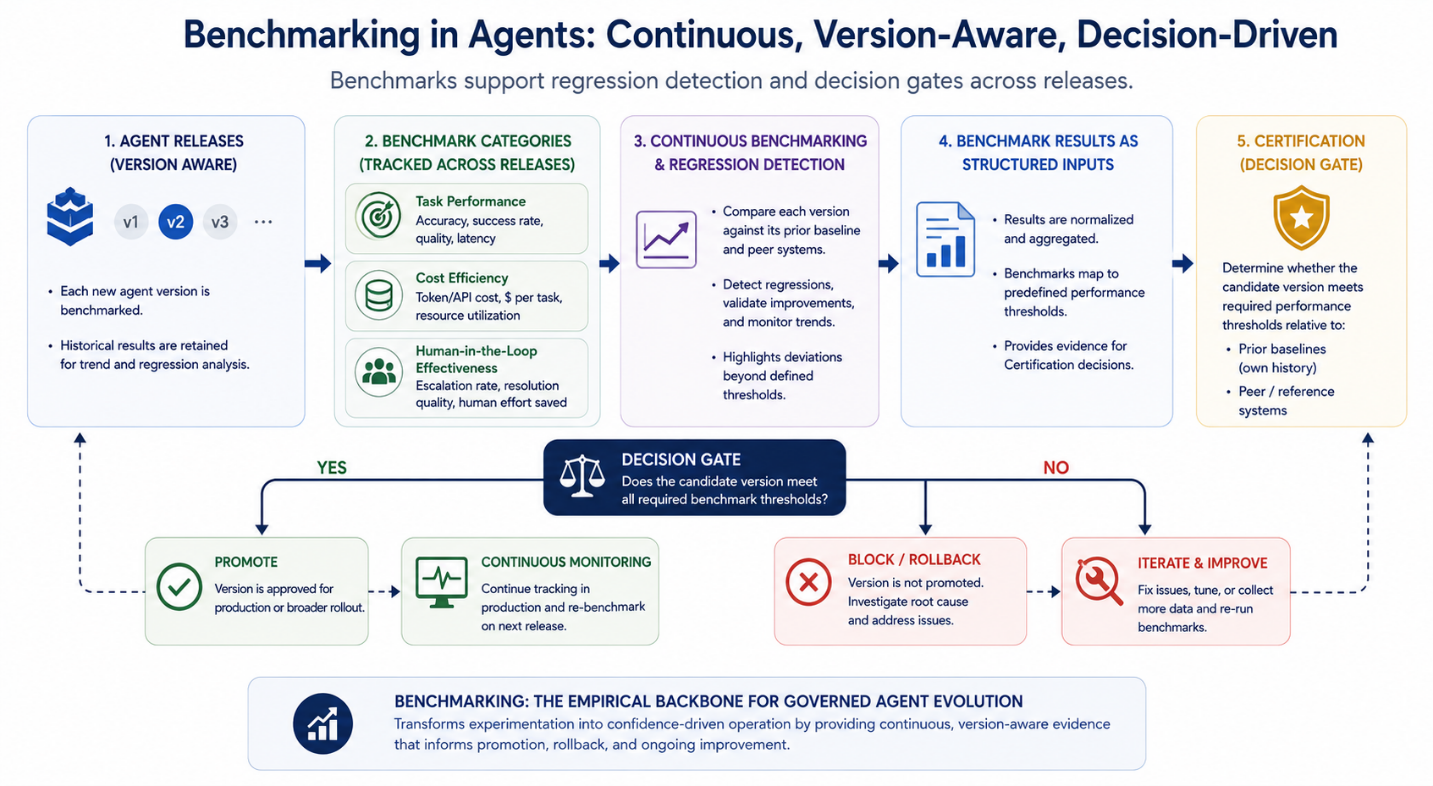
\includegraphics[width=0.9\textwidth]{figures/benchmarking/version-aware-benchmarking.png}
\caption{Continuous, version-aware, decision-driven benchmarking: regression detection and decision gates that feed into certification.}
\end{figure*}

\starttwocol

\section{The agent that quietly stopped working}

A maintenance-recommendation agent at a manufacturer scored 0.81 on the internal benchmark every Friday for nine months. Then, over the course of six weeks, the score quietly drifted down to 0.67. No one noticed. The dashboard had been green for so long that no one looked at it.

The cause turned out to be small. The team that owned one of the agent's tools --- a parts-availability lookup --- had updated its return-value format from a flat list to a structured object. The agent's prompt had been written for the flat-list version. It still mostly worked, because the agent was clever enough to handle the new format about 80\% of the time. The 20\% it failed on were rare diagnoses where the parts lookup mattered most. The benchmark caught the regression. No one read the benchmark.

This chapter is about the operational discipline that prevents that story. It is about running benchmarks on a cadence, tagging every score with what produced it, and noticing --- quickly and concretely --- when a number that has been stable starts to slip.

\section{Version-aware benchmarking and release gates}

A score on its own is information. A score tagged with what produced it is data. The difference is the discipline of \textit{version-aware benchmarking} --- every benchmark run records the model version, the prompt version, the tool versions, the data version, and the date. When the number changes, you know what could plausibly have caused it.

The point is not record-keeping for its own sake. The point is that any of those five things can change without your team initiating a change. The model can be updated by the vendor. A tool's behavior can shift when its underlying API does. The data the agent operates on (the customer base, the catalogue, the policy library) drifts. Without version tags, a regression is a mystery. With them, it is a triage.

For an agent in production, the right cadence is a benchmark run on every release (model update, prompt change, tool change) and on a fixed time interval (weekly or monthly, depending on stakes) regardless of whether anything has changed on your side. The fixed-interval runs are the ones that catch what changed on someone else's side.

\begin{TNdefinition}{Regression benchmark} a benchmark run on every release whose only purpose is to catch a worse model before it ships. The agentic equivalent of a unit-test gate. Distinct from the leaderboard-style benchmark, which is run occasionally and reported externally; a regression benchmark is run constantly and reported internally. \end{TNdefinition}

The release-gate version of this discipline is to refuse to promote a candidate agent to production until it passes the regression benchmark with a margin --- and to make ``with a margin'' precise enough that nobody argues about it the morning of release.

\section{Statistical sanity, formalized}

The single most-violated rule in continuous benchmarking is this: a two-point drop in a score is not necessarily a regression. A two-point gain is not necessarily an improvement. Both might be noise. Telling which is the difference between a team that ships good agents and a team that chases ghosts.

Here are the four ideas your team needs in their working vocabulary, each in one callout.

\begin{TNdefinition}{Confidence interval (bootstrap)} a way of expressing a benchmark score with its uncertainty attached. Resample the test cases with replacement many times (typically 1{,}000 or 10{,}000); recompute the score each time; the middle 95\% of those resampled scores is the 95\% confidence interval. Reporting ``82\%, 95\% CI [79\%, 85\%]'' instead of ``82\%'' honestly states what you know and what you don't. What this means for your decision: if two candidate agents' intervals overlap, the difference between them is not yet evidence; collect more data or accept that they tie. \end{TNdefinition}

\begin{TNdefinition}{Cohen's d (effect size)} a measure of how large the difference between two agents is, expressed in standard deviations rather than percentage points. The formula is \texttt{Cohen's d = (M1 - M2) / SD\_pooled}, where M1 and M2 are the two agents' mean scores and SD\_pooled is the pooled standard deviation of their score distributions. A d of 0.2 is ``small,'' 0.5 is ``medium,'' 0.8 is ``large.'' What this means for your decision: a statistically significant difference can still be too small to matter operationally. Cohen's d tells you whether to care. \end{TNdefinition}

\begin{TNdefinition}{Significance test (t-test, Mann-Whitney U, permutation)} three ways of asking whether the difference between two agents' scores is larger than you'd expect by chance. A t-test compares means and assumes the scores are roughly normally distributed; Mann-Whitney U makes weaker distributional assumptions; a permutation test makes the fewest assumptions of all by shuffling the labels many times to see how often a difference this large appears. For most benchmark comparisons, permutation tests are the safest default. What this means for your decision: if the test says p > 0.05, the difference you're looking at is consistent with noise, even if it looks meaningful. \end{TNdefinition}

\begin{TNdefinition}{Bonferroni / Benjamini-Hochberg correction} when you compare many things at once (every metric on the dashboard, every agent in the bake-off, every week's score against last week's), a few will look ``significantly different'' by chance alone. Bonferroni divides the significance threshold by the number of comparisons; Benjamini-Hochberg is a less aggressive version that controls the false discovery rate. What this means for your decision: if your team is comparing twenty metrics, the threshold for any one of them being a real finding is much stricter than 0.05. Without correction, the dashboard lies in slow motion. \end{TNdefinition}

The arithmetic is for your data scientists, not for Maya. The discipline is for everyone. Your team should report scores with intervals, compare scores with effect sizes, and apply a correction when they are running many comparisons at once. If they aren't, they are calling noise ``regression'' and noise ``improvement'' --- sometimes on the same week.

\begin{TNwarning} Without confidence intervals, every benchmark report is a story that confirms whatever the reader brought to it. The gold-standard fix is cheap: bootstrap the score distribution and report the interval next to the point estimate. Any team that won't is making decisions on something less than data. \end{TNwarning}

\section{Continuous benchmarking with humans in the loop}

For agents that operate with a human in the loop --- a customer-service agent handing off to a live representative, a triage agent flagging an exception for a clinician --- the benchmark you care about is not the agent's score in isolation. It is the score of the \textit{agent-plus-human system}. Chapter 4 names this; here is the operational version.

The signals to track are not the same as for an autonomous agent. They include the agent's intervention rate (how often a human has to step in), the agent's escalation accuracy (when it asks for help, is that the right call?), the time-to-resolution with the agent compared to a human-only baseline, and the post-intervention success rate. A \textit{higher accuracy} agent that doubles the intervention rate may reduce overall system effectiveness --- a sentence Maya should underline.

A useful exercise for any HiL agent is to benchmark the \textit{system} --- the agent and the human together --- on a representative slice of work, and compare it to the same slice handled by a human alone. If the agent-plus-human result is not meaningfully better than the human alone on outcomes and cost together, the agent is paying for itself with optics, not value.

\section{Leaderboard gaming --- the public secret}

Public leaderboards are useful. They are also gamed.

The gaming is not (usually) cheating in the obvious sense. It takes three forms, all of them legitimate-looking, and all of them corrosive to using a leaderboard score as a signal.

\textbf{Overfitting to the benchmark.} A team trains, evaluates, and retrains until the model does well on a particular benchmark, at the cost of generalization. The score goes up. The agent does not get better at anything that isn't on the benchmark.

\textbf{Test set contamination.} Benchmarks are public; training data is huge; the test set ends up in the training data, deliberately or otherwise. The score goes up. The model has memorized rather than learned.

\textbf{Methodology arbitrage.} A vendor runs the benchmark with a kinder configuration than competitors --- more attempts, a more permissive scoring rule, a private fork that drops the hardest cases. The score goes up. The number is no longer comparable to anyone else's.

The defenses are familiar from \autoref{ch:30-benchmarking-10-capability}: treat any sudden jump as a question, ask for the methodology, run your own held-out tests on data the vendor has never seen. The longer-term defense is to weight your decision on your own evaluations --- Part IV territory --- over any public number, however prestigious.

The deeper rule is Goodhart's Law, the social-science observation that ``when a measure becomes a target, it ceases to be a good measure.'' Every leaderboard becomes a target the moment it matters. Treat the leaderboard score as a screening signal, not a deciding one.

\section{The vignette that closes Part III}

\begin{TNinpractice}{Helix Health} \textit{A regional health system running a clinical-coding agent that had scored within 1\% of its golden-dataset baseline every release for six months.} The most recent model upgrade dropped the score by 4\%. The team's first instinct was to call it noise. The on-call data scientist ran a bootstrap on the result and the 4\% gap was outside the confidence interval --- real, not noise. The drop turned out to be concentrated in rare diagnosis codes, the ones the golden dataset undersampled. The benchmark had been stable for six months because it had been testing the wrong slice. The fix was not to roll back the model. The fix was to expand the regression benchmark to include the rare-code distribution, run a recertification, and tag the new score as the v2 baseline. Two weeks of work; the agent stayed in production. Without version-aware tracking and a confidence interval, the team would either have shipped the regression or rolled back unnecessarily, and would not have known which. \end{TNinpractice}

The benchmark caught what the team thought to look at. The evaluation caught what the benchmark missed. That is the bridge from Part III to Part IV.

\section{When to retire a benchmark}

A benchmark earns its place by predicting production behavior. When it stops predicting --- because the model class has moved past it, because the test set leaked into training data, because the use case shifted under it --- it stops being useful and starts being misleading. The benchmarks your team trusted in 2023 are not the benchmarks worth running in 2026, and the discipline of noticing the difference is its own skill.

Three sunset signals are worth naming.

\textbf{Saturation.} Every credible agent now scores in the top 5\% on the benchmark. The numbers crowd into a band that is narrower than the noise on any one of them, and the benchmark is no longer differentiating. A score at the top of a saturated benchmark tells you the agent is competent at a problem the field has solved; it does not tell you which agent to pick.

\textbf{Drift from production.} Improvements on the benchmark stop correlating with improvements your team observes in production. A new release climbs two points on the public board and changes nothing your operators can feel; a release that drops a point ships a meaningful gain on your own traffic. The benchmark and the job have parted ways. When this happens repeatedly, the benchmark is measuring something your work no longer is.

\textbf{Contamination beyond rescue.} The benchmark's test set has leaked into model training data so thoroughly that no agent can be evaluated against it honestly. The SWE-bench to SWE-bench Verified migration was a clean version of this story --- the community accepted that the original was compromised and built a successor. Most benchmarks do not get that treatment; they quietly stop being trustworthy and keep being cited.

\begin{TNdefinition}{Benchmark sunset} the retirement of a benchmark from the decision-making suite. Sunset is terminal: distinct from rotation, where the benchmark gets refreshed and stays in use. \end{TNdefinition}

The evaluation framework chapter (\autoref{ch:40-evaluation-14-framework}) covers when to refresh internal golden datasets; this chapter is about when to retire \textit{public} benchmarks. Both run on quarterly review at minimum.

\section{Where benchmarking stops and evaluation starts}

Benchmarking compares. Evaluation answers. Benchmarking is shared; evaluation is yours. Benchmarking gives you the language to read a vendor's deck and a model release note. Evaluation gives you the language to know whether your agent is doing the job you hired it for, on your data, today.

Chapter 13 draws the full distinction. The short version: when Maya's auditor asks ``is this benchmark report enough?'' the answer is no, and the rest of the book is about what is.

\TNrule

\stoptwocol

\begin{TNkeytakeaways}
\item Benchmark every release and on a fixed interval. The interval is what catches what changed outside your control.
\item Tag every score with model, prompt, tool, data, and date versions. Without tags, regressions are mysteries.
\item A two-point change is noise until proven otherwise. Confidence intervals and effect sizes are the proof.
\item For human-in-the-loop agents, benchmark the system (agent plus human), not the agent alone.
\item Treat public leaderboard scores as screening signals, not deciding ones; everything that gets gamed eventually does.
\end{TNkeytakeaways}

\begin{TNchecklist}
\item Implement a regression benchmark that runs automatically on every release and on a fixed weekly or monthly cadence.
\item Tag every benchmark run with model version, prompt version, tool versions, dataset version, and date.
\item Require confidence intervals or score distributions on every benchmark report your team produces.
\item Apply a multiple-comparison correction (Bonferroni or Benjamini-Hochberg) when reporting many metrics together.
\item For any agent with a human in the loop, define the system-level KPI (agent+human outcomes) and benchmark that, not the agent alone.
\item Pair every public leaderboard score in any vendor comparison with a result from a held-out internal test the vendor has not seen.
\item Schedule a quarterly review specifically of ``what changed in the benchmarks themselves'' --- benchmarks are not static infrastructure.
\end{TNchecklist}



